\documentclass{beamer}

\usepackage[beamer]{shortcut}
\graphicspath{{./images/}{/home/tom/Pictures/Logos/}}

\def\biblio{
    \nobibliography{../../../library}
    \def\biblio{}
}

\institute{INRIA Saclay}
\author{Thomas Moreau}
\title{
    Impact of Open Source Software\\
    in Research
}

\setbeamertemplate{title page}[frame]
\def\extraLogo{}
\def\LOGOS{
% \includeLogos[1em]{logo_mind_big,logo_EULPS,logo_inria}\\[.5em]
    \hskip-1em
    \raisebox{-1.5em}{
\includegraphics[height=3em]{logo_inria}}
    \hskip2em
    \raisebox{-2em}{\includegraphics[height=4em]{logo_mind}}
    \hskip2em
    \raisebox{-2.5em}{\includegraphics[height=5em]{logo_cea}}\\[.5em]
}

\begin{document}

\begin{frame}
    \titlepage
    % \biblio{}
\end{frame}

% \begin{frame}{Agenda}
%     \myitem{} Reminder of the team contribution to OSS\\
%     \myitem{} Benefit from OSS\\
%     methods are reused, more visibility/citations, more robust tools,\\
%     \myitem{} Challenges from OSS\\
%     maintainance takes time, technical and cognitive debts, harder to put visibility in academia?
% \end{frame}

\frame{
    \frametitle{Core ML Libraries}

    \begin{columns}
        \column{.3\textwidth}
        \centering
        \includegraphics[width=\textwidth]{logo_sklearn}\\
        \column{.3\textwidth}
        \centering
        \includegraphics[width=.7\textwidth]{logo_joblib}\\[1em]
        \includegraphics[width=.7\textwidth]{logo_loky}\\
        \column{.3\textwidth}
        \centering
        \includegraphics[width=\textwidth]{logo_benchopt}\\
    \end{columns}
}

\frame{
    \frametitle{Domain Specific Software}

    \textbf{Maintainers:}\\
    \begin{columns}
        \column{.3\textwidth}
        \centering
        \includegraphics[width=.9\textwidth]{logo_mne}\\
        \column{.3\textwidth}
        \centering
        \includegraphics[width=.6\textwidth]{logo_nilearn}\\
        \textbf{NiLearn}\\[2em]
        \textbf{\Large NeuroLang}
        \column{.3\textwidth}
        \centering
        \includegraphics[width=.7\textwidth]{logo_pysap-mri}\\
    \end{columns}
    \vskip2em


    \textbf{Contributors:}\\[1em]
    \begin{columns}
        \column{.3\textwidth}
        \centering
        \includegraphics[width=\textwidth]{logo_braindecode}\\
        \column{.3\textwidth}
        \centering
        \includegraphics[width=1.2\textwidth]{logo_deepinv}\\
        \column{.3\textwidth}
        \centering
        \includegraphics[width=.7\textwidth]{logo_moabb}\\
    \end{columns}
}

\frame{
    \frametitle{Research Software}

    \textbf{Consolidating research results:}\\[1em]
    \begin{columns}
        \column{.3\textwidth}
            \centering
            \Large DicoDile\\[1em]
            FaDIn\\
        \column{.3\textwidth}
            \centering
            \includegraphics[width=.7\textwidth]{brain_and_signals}\\
            \Large\texttt{{\color{orange}$\pmb\alpha$}csc}
        \column{.3\textwidth}
            \centering
            \Large MRI-NUFFT\\[1em]
            \Large FuGW
    \end{columns}


    \vskip3em
    \textbf{Code for our research papers:}\\[1em]
    \myitem{} Many repo to reproduce our experiments,\\[.5em]
    \myitem{} Now a standard practice in ML community.\\
}

\frame{
    \frametitle{Benefits of the Software Publication}

    \textbf{Improve Research:}\\[1em]
        \myitem{} Improve reproducibility,\\[.5em]
        \myitem{} Push for fair benchmarks,\\[.5em]
        \myitem{} Make methods more robust.\\[2em]

    \textbf{Increase Impact of the Team}\\[1em]
        \myitem{} Developed methods are reused,\\[.5em]
        \myitem{} More visibility: citations/collaborations.\\[2em]

    \emph{Often a good ground for interactions with other teams.}
}

\frame{
    \frametitle{Challenges of the Software Publication}

    \textbf{Burden of maintaining many softwares:}\\[1em]
        \myitem{} Many published repos lead to high maintenance burden,\\[.5em]
        \myitem{} High cognitive load and technical debt.\\

    \strongpoint{Need to gather the efforts!}
    \vskip2em

    \textbf{Academic recognition:}\\[1em]
        \myitem{} Maintaining software takes time,\\[.5em]
        \myitem{} Academic credit can be challenging.\\

    \strongpoint{Need to have support of our institutions!}
    \vskip1em
    \emph{and a good strategy.}

}

\frame{
    \frametitle{PEPR NumPEx -- building software for Exascale}


    \textbf{Context:} First exascale machine will be delivered in 2026.
    \strongpoint{Need to prepare softwares to run on it!}

    \vskip3em
    \textbf{Team involvement}\\[1em]
    \myitem{} Adapting \texttt{scikit-learn} and \texttt{joblib} to leverage HPC.\\[.5em]
    \myitem{} Developping methods to process simulation results.\\[.5em]

    \strongpoint{Aggregating efforts for large scale signals processing with ML!}

    \vskip2em
    \emph{}
}

%%%%%%%%%%%%%%%%%%%%%%%%%%%%%%%%%%%%%%%%%%%%%%%%%%%%%%%%%%%%%%%%%%%%%%%%%%%%%%%
\begin{frame}[fragile]{Benchopt \rightcite{Moreau et al. 2022}}

    Reproducing this comparison and adding solvers and tasks is easy as:\\[.5em]


    \begin{center}
    \begin{tabular}{c}
\begin{lstlisting}[language=bash,linewidth=.78\textwidth]
git clone https://github.com/benchopt/benchmark_bci
benchopt run ./benchmark_bci
\end{lstlisting}
    \end{tabular}
    \end{center}

    \vskip.5em\centering
    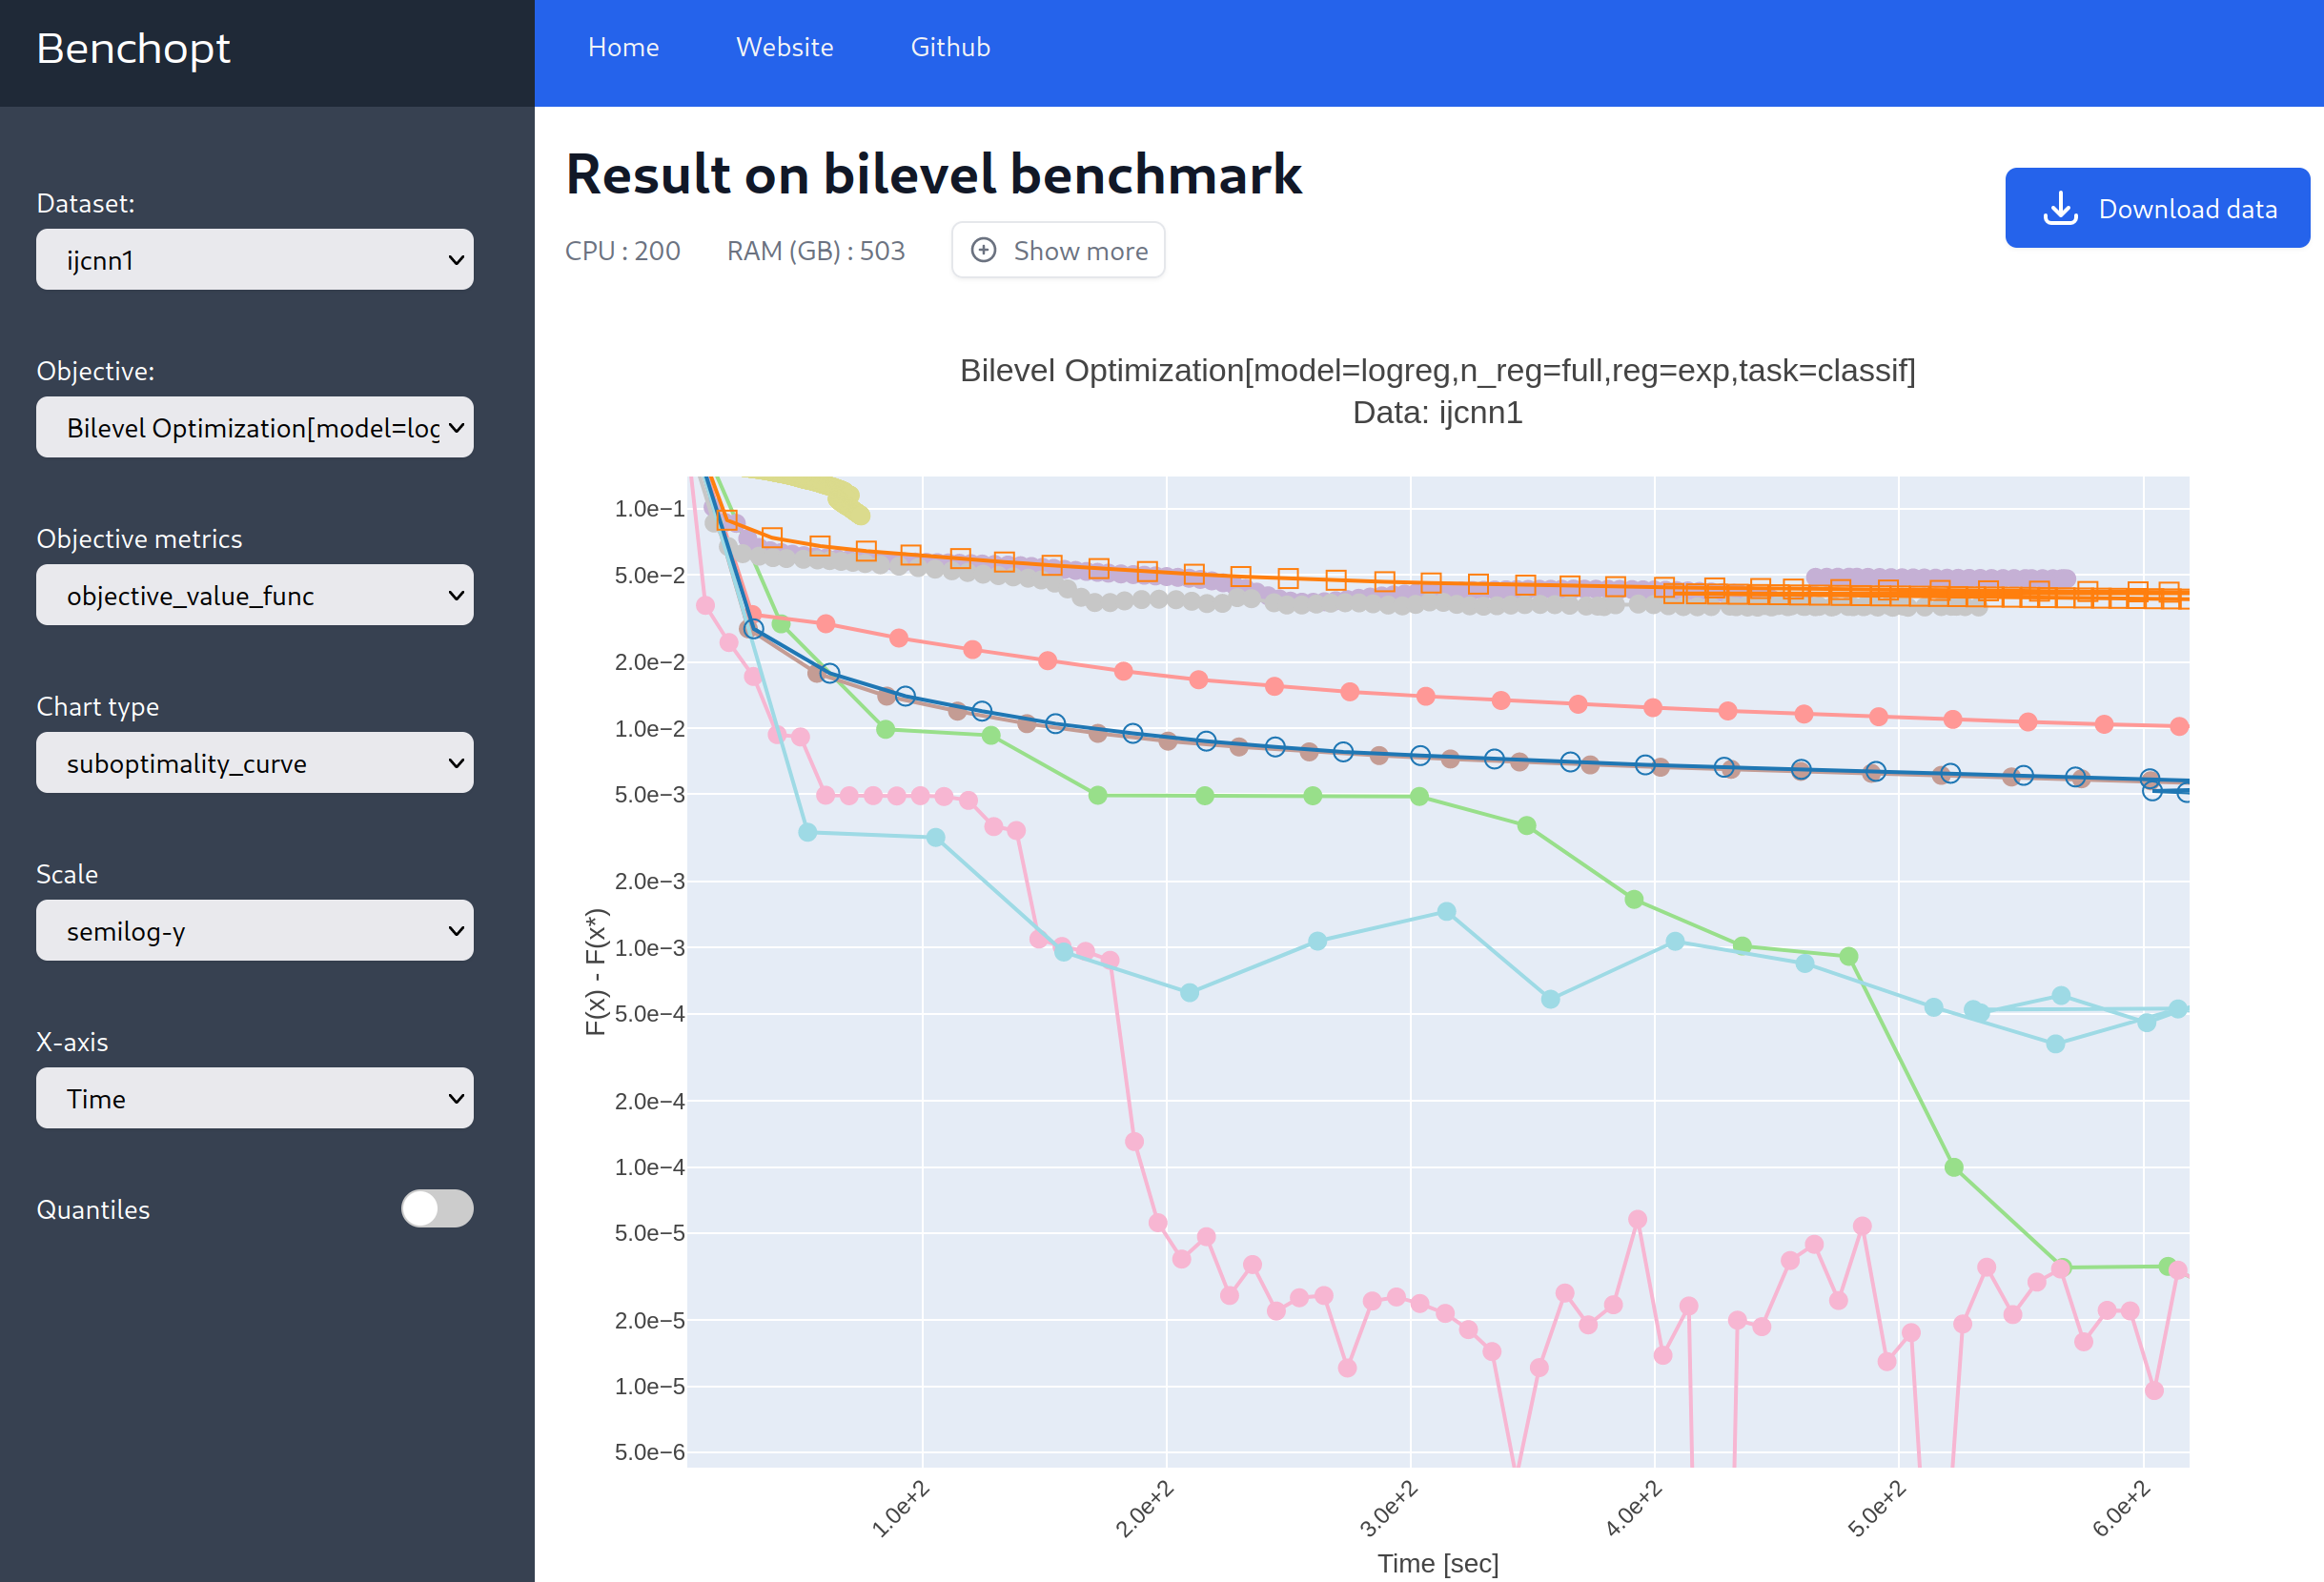
\includegraphics[width=.7\textwidth]{benchopt_bilevel}\\

    % \hskip3ex
    % 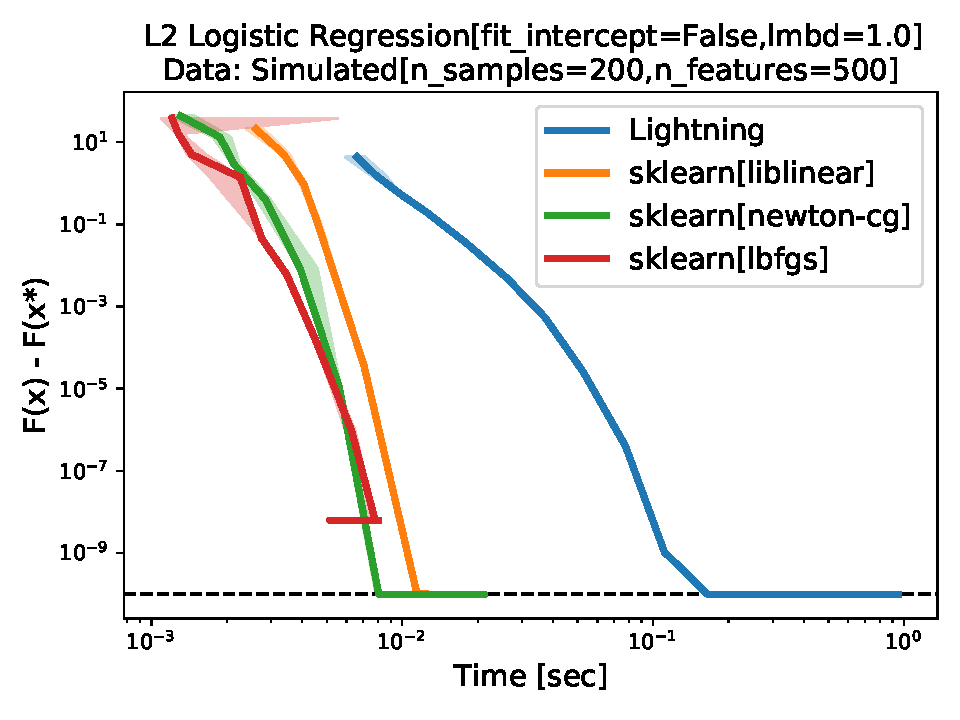
\includegraphics[width=.45\textwidth]{logreg_l2_1}

\end{frame}
%%%%%%%%%%%%%%%%%%%%%%%%%%%%%%%%%%%%%%%%%%%%%%%%%%%%%%%%%%%%%%%%%%%%%%%%%%%%%%%

% %%%%%%%%%%%%%%%%%%%%%%%%%%%%%%%%%%%%%%%%%%%%%%%%%%%%%%%%%%%%%%%%%%%%%%%%%%%%%%%
% \frame{
%     \frametitle{Benchopt: principle}

%     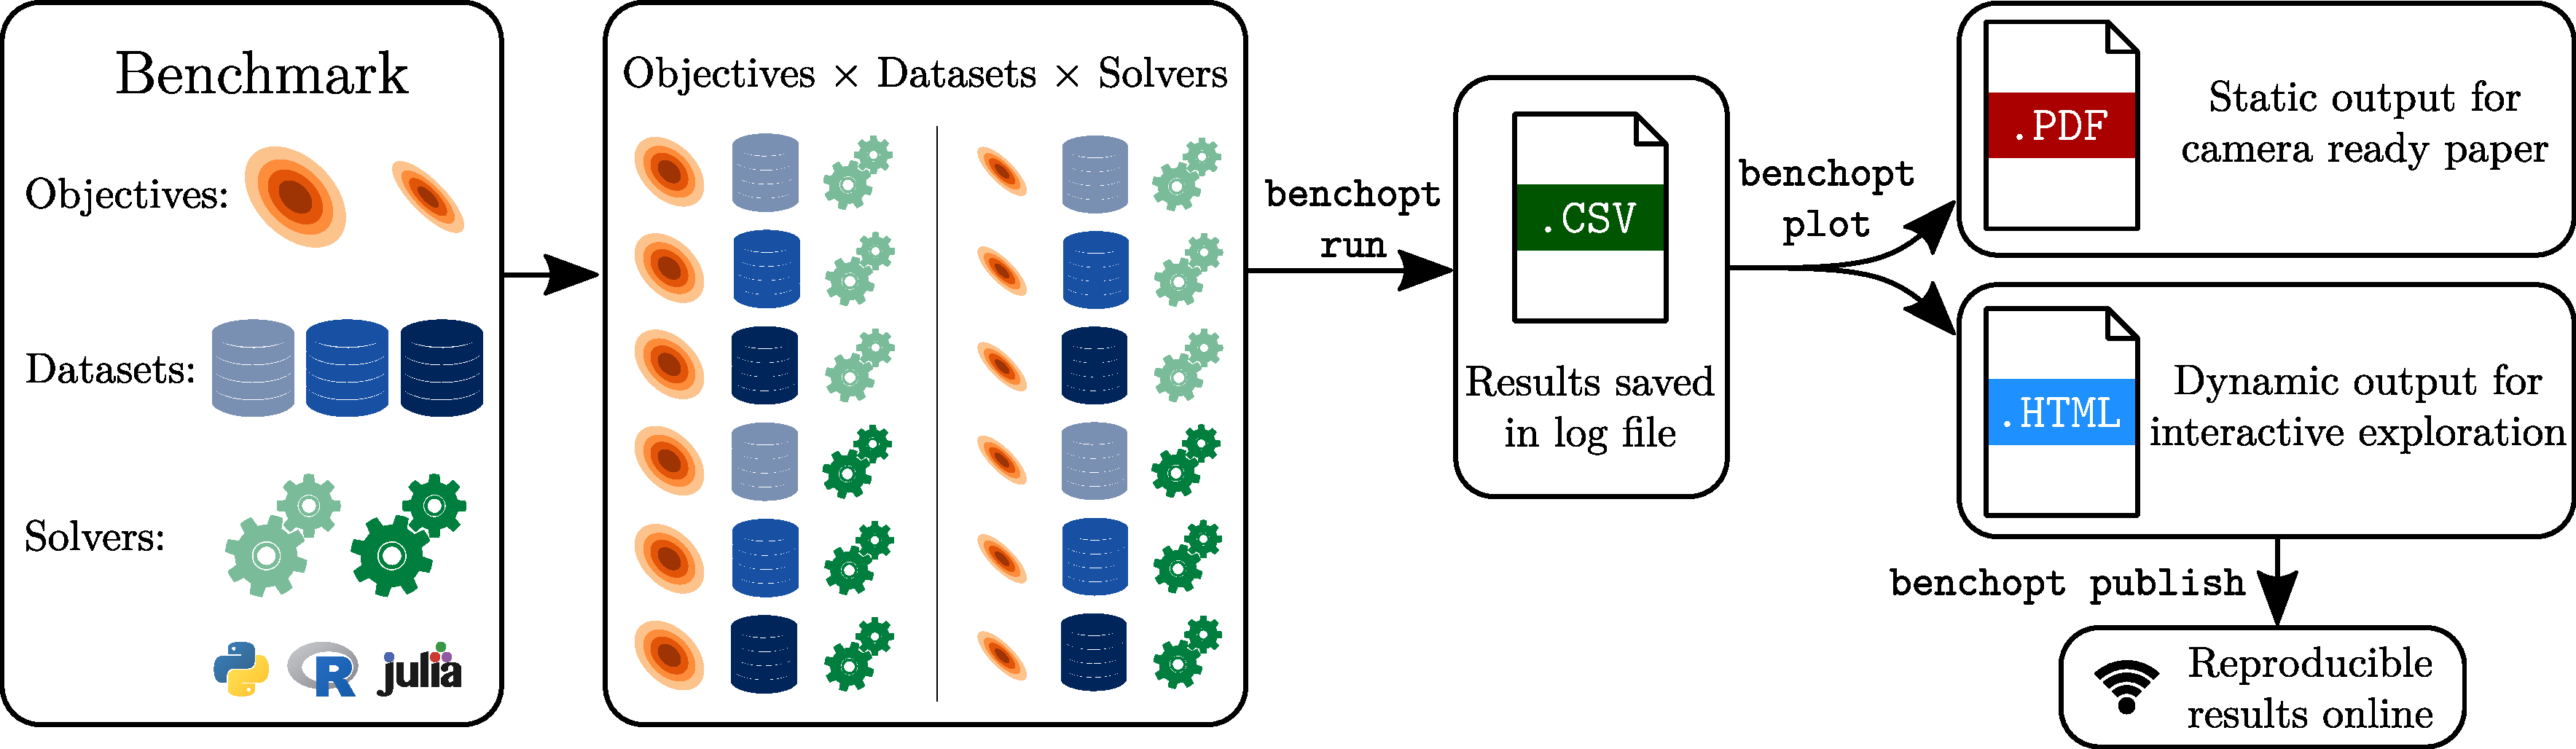
\includegraphics[width=\textwidth]{benchopt_schema_objectives_with_logos}

%     \strongpoint{Each object can be parametrized so multiple scenario can be tested.}

%     \vskip1.5em
%     \textbf{Making tedious tasks easy:}\\[1em]
%     \centering

%     \myitem{} Sharing code
%     \hskip3ex \myitem{} Adding methods
%     \hskip3ex \myitem{} Exploring results\\[.5em]
%     \myitem{} Varying hyperparameters
%     \hskip3ex \myitem{} Running in Parallel
%     \hskip3ex \myitem{} Caching\\[.5em]
%     \hskip-4em\myitem{} \dots
% }


%%%%%%%%%%%%%%%%%%%%%%%%%%%%%%%%%%%%%%%%%%%%%%%%%%%%%%%%%%%%%%%%%%%%%%%%%%%%%%%


\frame{
    \frametitle{Benchopt's benchmarks for neuroscience}

    {\centering\includegraphics[height=.3\textheight]{logo_benchopt}\\[2em]}

    \begin{columns}[T]
        \column{.5\textwidth}
        \myitem{} Brain-Computer Interface,\\[1em]
        \myitem{} Brain-age prediction,\\[1em]
        \myitem{} Brain alignment,\\[1em]
        \myitem{} MRI reconstruction,\\[.5em]
        \strongpoint{Add yours!}
        \column{.5\textwidth}
        \centering
        
\includegraphics[width=.8\textwidth]{sprint1}\\
        Benchopt sprint in July.
    \end{columns}
}

\end{document}